%\begin{itemize}
%  \item Explain NUMA, and that in TBB with use only 1 NUMA node
%  \item Try of NUMA interleaved with TBB
%  \item Explain memory distribution of schema
%  \item NUMA management improve perf but not enough
%\end{itemize}

In this section, we further improve on the previous results by taking into
account the NUMA (Non Uniform Memory Access) characteristics of the
testbed machine: Both 4-core sockets have a faster access to their
own memory bank than to the opposite socket's memory bank (Fig. \ref{fig:alloc_numa}).

\begin{figure}[!t]
  \centering
  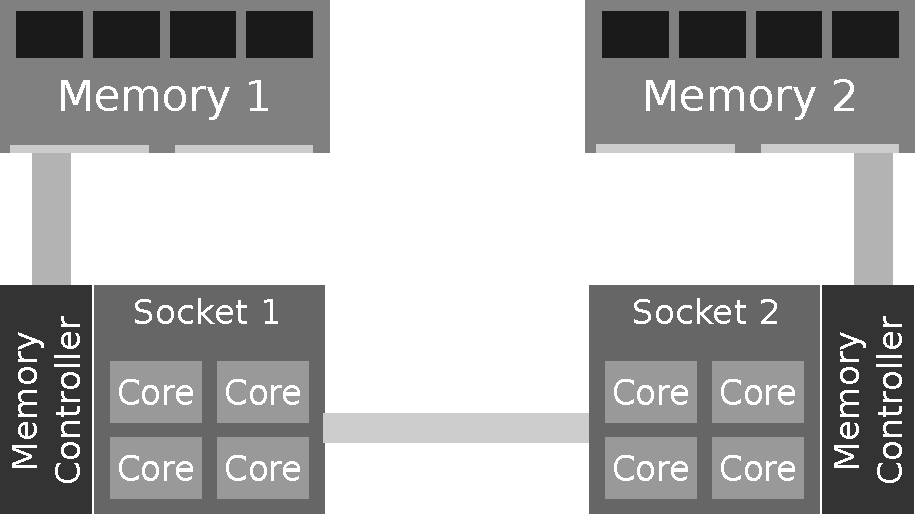
\includegraphics[width=3in]{alloc_numa_nb}
  \caption{NUMA Machine with 2 sockets of 4 cores}
  \label{fig:alloc_numa}
\end{figure}

In a general way, a program allocates memory from a virtual address space
split into pages. Each page used by the program is transparently
mapped to a physical memory location. Thus, some virtual pages can
also be moved from one physical location to another one, while the
virtual/physical mapping is transparently updated accordingly to the
operating system without affecting the execution of user level
programs. However, the physical location of virtual page may
impact the program performance on NUMA architectures, depending on the
connectivity between the physical memory bank where a page is
located and the socket core that is accessing this memory bank.

The NUMA memory allocation policy is defined by the operating system.
With Linux, at least the following three memory policies are generally available:
% CR: Add ``based operating systems'' after Linux ?
\begin{itemize}
\item {\em First Touch}: Memory is allocated on the bank next to
  the core which accessed the data first. This is the default policy.
\item {\em Bind}: Memory is allocated on a specific bank.
\item {\em Interleaved}: Memory allocations are interleaved among
  all the banks available.
\end{itemize}
On Linux, these policies can be set either through the
\textit{mbind} system call, or with the {\em numactl} command line tool.

Other operating system may come with their own specific sets of NUMA
memory allocation policies. Solaris, for instance, also provides the
\textit{next-touch}~\cite{next_touch}
% ST: TODO: Le papier de Brice & Nathalie n'est pas vraiment le mieux
% pour mentionner quelque chose de Solaris...
% CR: J'ai remplacé la citation par l'article cité par Brice & Nathalie dans \cite{GoFu09Next-touch}.
policy. When this policy is
selected, a memory page is moved to the bank close to
the core that subsequently accesses it.

%-------------------------------
\subsection{Interleaved Memory Allocation Policy}\label{subsec:numa_inter}
When the interleaved policy is selected, Linux uniformly distributes
newly allocated physical pages among all available NUMA banks,
following a round robin scheme. While having very little impact on the
applicative code, the interleave policy often shows some effectiveness
in mitigating NUMA overheads in the general case, because it
distributes the required memory bandwidth over the various memory banks.
Thus, it is usually
worthwhile to experiment with it, before investigating the NUMA issue
further.

The following tables show the performance results obtained after
enabling the interleaved memory allocation policy. We first test this
method using Intel TBB as the low-level runtime under the Taggre layer described in previous section
(Tables~\ref{tab:full:8:facto:no}~to~\ref{tab:full:8:solve:nested}).



While the results we obtain show an improved speed-up with TBB and interleaved policy,
it should be noted that sequential runs with interleaved policy are of
course worse, because of memory access penalties introduced by NUMA.
%% Parallel runs however show a better speed-up.
When comparing
interleaved page allocation with first-touch allocation, we get
an average improvement of 3.5\,\% on ILU(k) preconditioner
and 6.2\,\% on triangular solve with two 4-core sockets.

\begin{table}[!h]
  \renewcommand{\arraystretch}{1.3}
  \caption{Results on the ILU(k) factorization step on two 4-core sockets in natural ordering.}
  \label{tab:full:8:facto:no}
  \centering
  \begin{tabular}{|c|c||c|c|c|}
    \hline
    Matrix & ILU & TBB & TBB interleaved & Nas\\
    &     &  \multicolumn{3}{c|}{speed-up}\\
    \hline
    \hline
    & ILU(0) &            2.54  &  2.68  &  2.80\\
    CUBE\_100 & ILU(1) & 3.79  &  3.86  &  3.95\\
    & ILU(2) &            3.91  &  5.82  &  {\bf 6.19}\\
    \hline
    & ILU(0) &            3.78  &  5.10  &  5.34\\
    SPE10 &     ILU(1) &  5.72  &  5.84  &  6.64\\
    & ILU(2) &            6.21  &  6.34  &  {\bf 6.84}\\
    \hline
  \end{tabular}
\end{table}

\begin{table}[!h]
  \renewcommand{\arraystretch}{1.3}
  \caption{Results on the ILU(k) preconditioner step on two 4-core sockets in nested dissection ordering.}
  \label{tab:full:8:facto:nested}
  \centering
  \begin{tabular}{|c|c||c|c|c|c|}
    \hline
    Matrix & ILU & TBB & TBB interleaved & Nas\\
    &     &  \multicolumn{3}{c|}{speed-up}\\
    \hline
    \hline
    & ILU(0) &            3.31  &  3.65  &  3.95\\
    CUBE\_100 & ILU(1) &  4.77  &  4.90  &  5.14\\
    & ILU(2) &            5.46  &  5.54  &  {\bf 5.72}\\
    \hline
    & ILU(0) &            3.09  &  3.70  &  4.00\\
    SPE10     & ILU(1) &  5.00  &  5.01  &  5.57\\
    & ILU(2) &            5.57  &  5.62  &  {\bf 6.06}\\
    \hline
  \end{tabular}
\end{table}



\begin{table}[!h]
  \renewcommand{\arraystretch}{1.3}
  \caption{Results on the Triangular Solve step on two 4-core sockets in natural ordering.}
  \label{tab:full:8:solve:no}
  \centering
  \begin{tabular}{|c|c||c|c|c|c|}
    \hline
    Matrix & ILU & TBB & TBB interleaved & Nas\\
    &     &  \multicolumn{3}{c|}{speed-up}\\
    \hline
    \hline
    & ILU(0) &            2.44  &  3.51  &  2.66\\
    CUBE\_100 & ILU(1) &  2.82  &  3.68  &  2.95\\
    & ILU(2) &            2.98  &  {\bf 3.76}  &  3.18\\
    \hline
    & ILU(0) &            2.52  &  3.58  &  3.24\\
    SPE10     & ILU(1) &  3.77  &  4.04  &  4.43\\
    & ILU(2) &            4.14  &  4.41  &  {\bf 4.96}\\
    \hline
  \end{tabular}
\end{table}

\begin{table}[!h]
  \renewcommand{\arraystretch}{1.3}
  \caption{Results on the Triangular Solve step on two 4-core
    sockets with TBB and interleaved allocation with nested dissection.}
  \label{tab:full:8:solve:nested}
  \centering
  \begin{tabular}{|c|c||c|c|c|c|}
    \hline
    Matrix & ILU & TBB & TBB interleaved & Nas\\
    &     &  \multicolumn{3}{c|}{speed-up}\\
    \hline
    \hline
    & ILU(0) &            1.67  &  2.11  &  1.92\\
    CUBE\_100 & ILU(1) &  1.92  &  2.25  &  2.07\\
    & ILU(2) &            2.08  &  {\bf 2.42}  &  2.24\\
    \hline
    & ILU(0) &            1.82  &  2.26  &  2.19\\
    SPE10     & ILU(1) &  2.71  &  2.82  &  3.08\\
    & ILU(2) &            2.90  &  3.01  &  {\bf 3.32}\\
    \hline
  \end{tabular}
\end{table}

These improvements could be further enhanced by taking into account the locality of data 
used by tasks within the task scheduler. This is the purpose of the
following section.
